%% AlpacaVision AI — Supplementary Material for MDPI Animals
%% Compile: pdflatex supplementary.tex
\documentclass[11pt,a4paper]{article}
\usepackage[margin=2.4cm]{geometry}
\usepackage{graphicx}
\usepackage{caption}
\usepackage[hidelinks]{hyperref}
\graphicspath{{../figures/}}
\renewcommand{\thefigure}{S\arabic{figure}}
\captionsetup{labelfont=bf}

\title{\vspace{-1.5cm}Supplementary Material\\[4pt]
\large Automatic Detection of Morphological Anomalies in Altiplano Alpacas Using a
Computer Vision System: A Curated Dataset, Compact Detector, and Ocular Anomaly
Classification Feasibility Study}
\author{Vilca-Sol\'orzano, R.A.; Yana-Yucra, D.M.; Ccopa-Acero, C.D.; Alem\'an-Gonzales, L.}
\date{}

\begin{document}
\maketitle
\vspace{-0.8cm}

\noindent These figures provide detailed diagnostics for the ocular-anomaly-classifier
feasibility study (Section~3.2 of the main text). Because the leakage-free classifier
performs at chance (AUC-ROC~=~0.506, 95\% CI [0.366, 0.645]), they are reported here as
supporting evidence of the negative result rather than in the main text.

\begin{figure}[h]
  \centering
  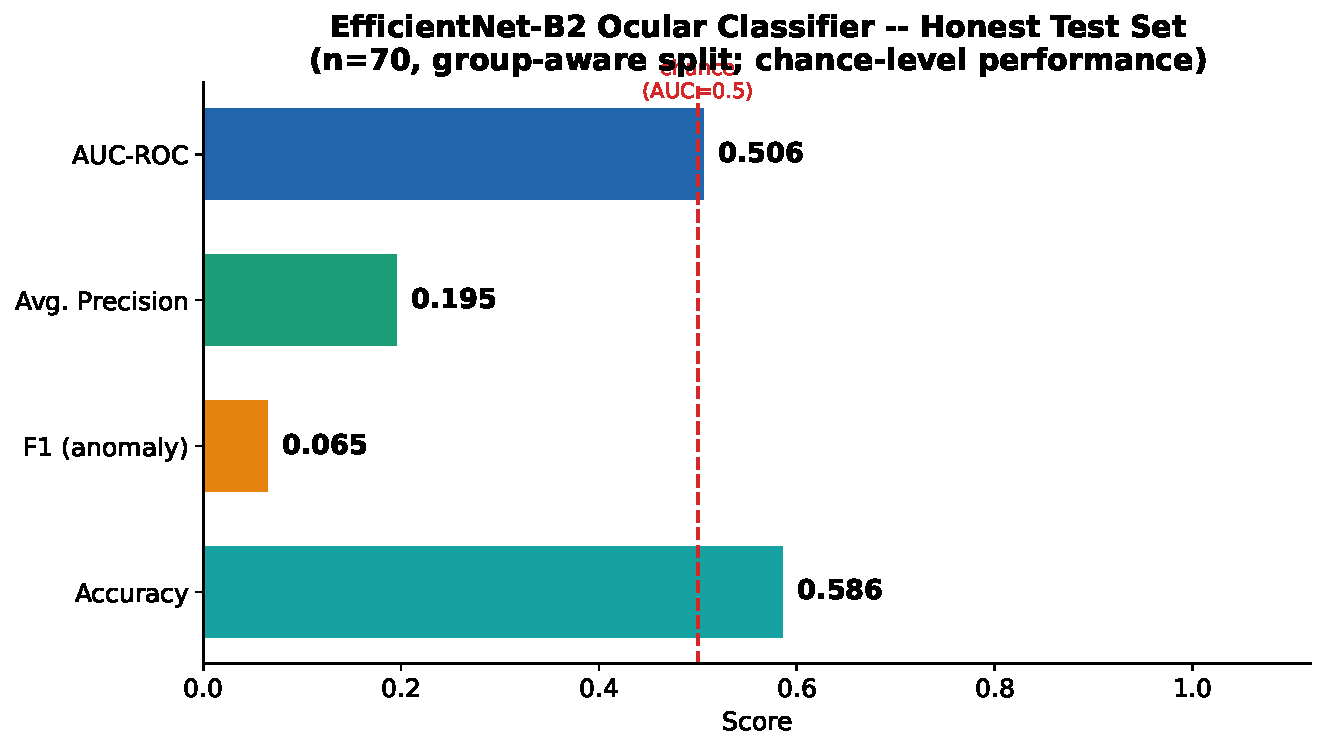
\includegraphics[width=0.85\textwidth]{fig4_classifier.pdf}
  \caption{EfficientNet-B2 ocular anomaly classifier: leakage-free test-set metrics
           ($n=70$, group-aware split). AUC-ROC~=~0.506 sits on the chance line (dashed),
           with Average Precision~=~0.195, F1~(anomaly)~=~0.065 and Accuracy~=~0.586.}
\end{figure}

\begin{figure}[h]
  \centering
  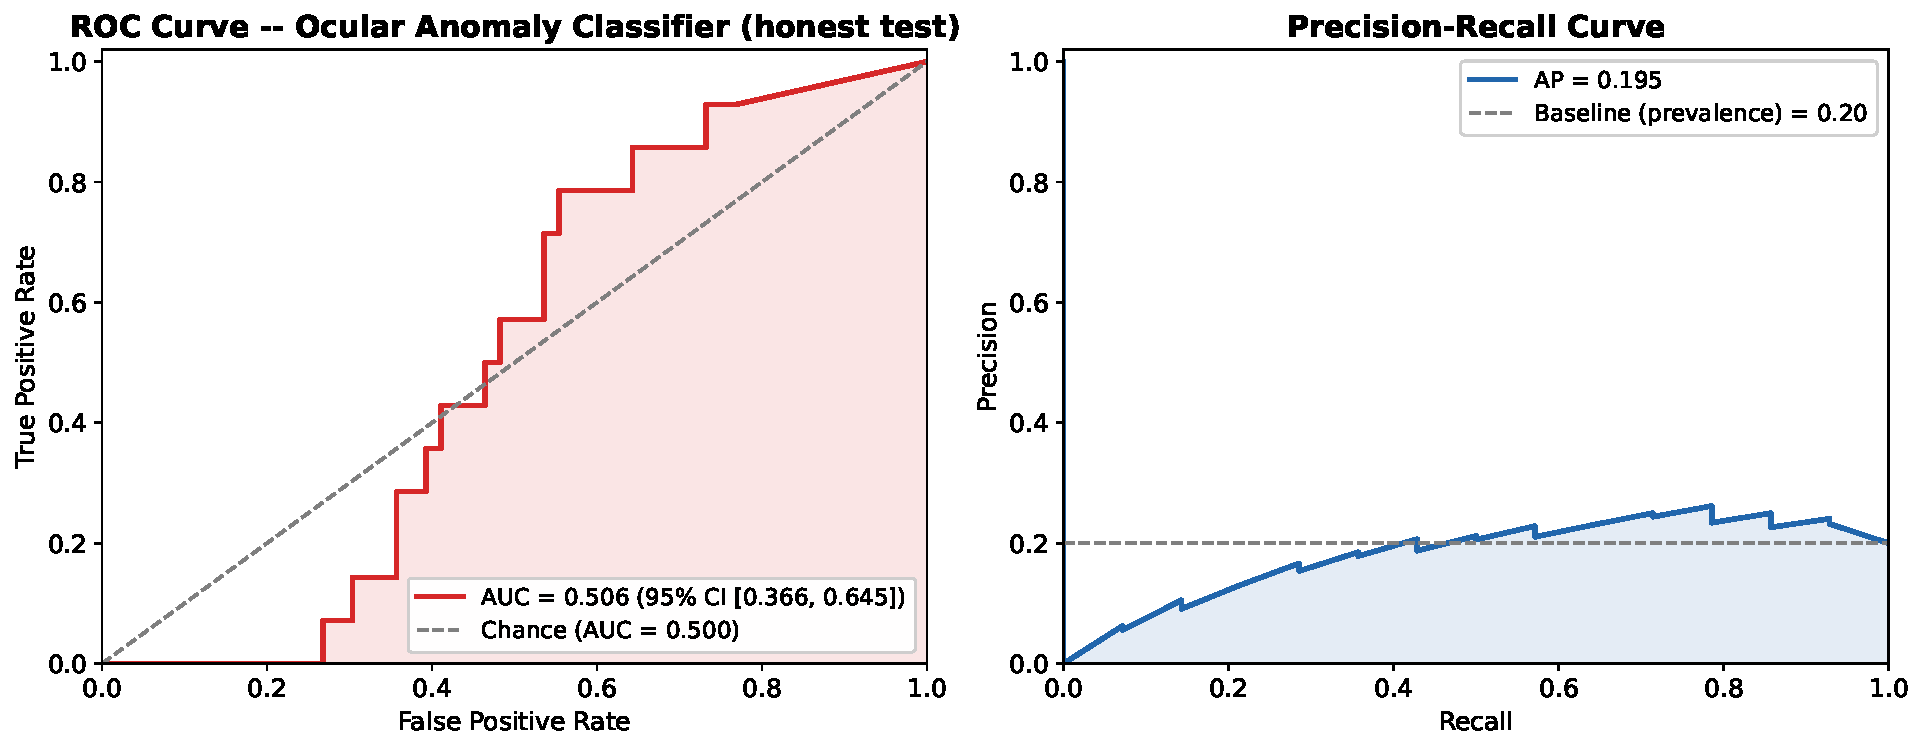
\includegraphics[width=\textwidth]{fig7_roc_pr.pdf}
  \caption{ROC and precision--recall curves for the classifier under the leakage-free
           protocol (bootstrap $B=1000$, seed~=~42). The ROC lies on the chance diagonal
           (AUC~=~0.506); the PR curve tracks the prevalence baseline (AP~=~0.195).}
\end{figure}

\begin{figure}[h]
  \centering
  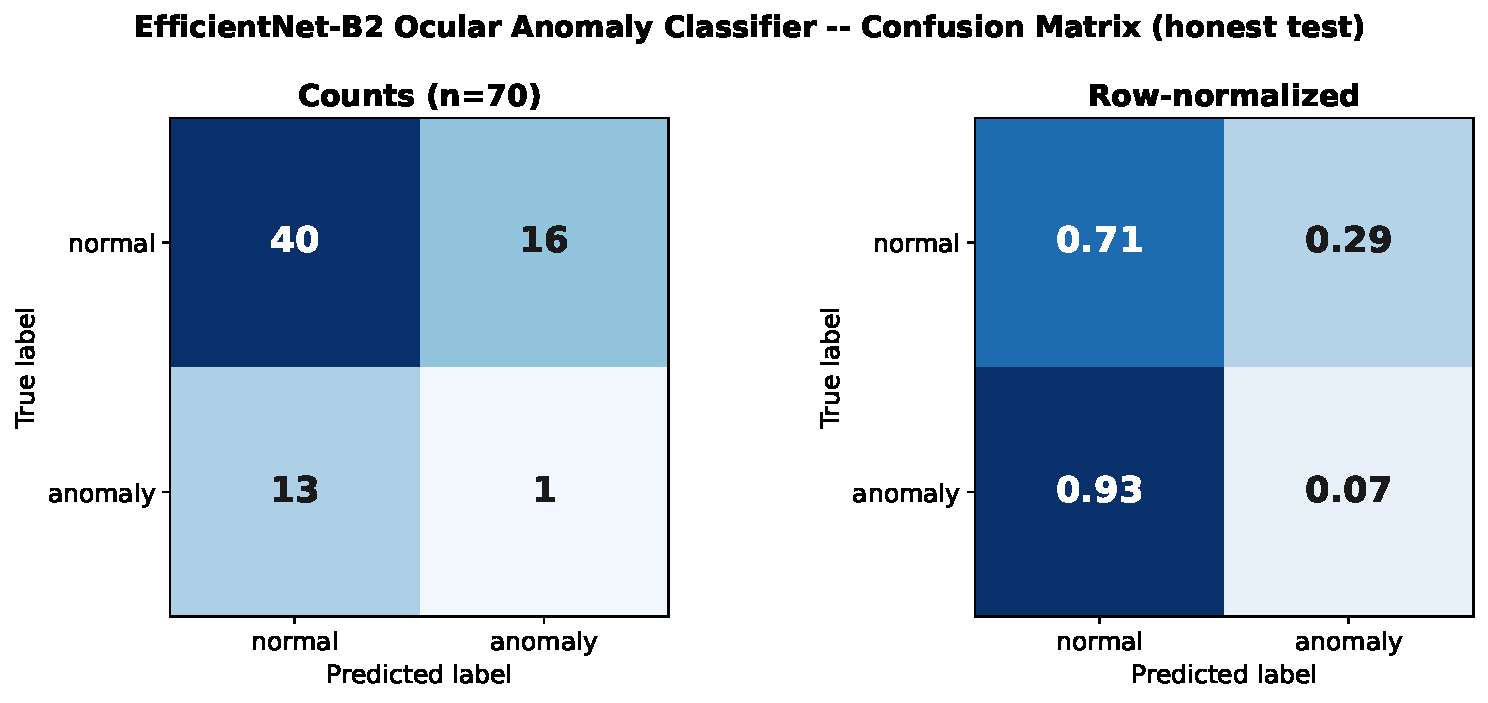
\includegraphics[width=0.9\textwidth]{fig9_confusion_matrices.pdf}
  \caption{Confusion matrices for the classifier: raw counts (left, $n=70$) and
           row-normalised (right). Of 14 true anomalies only 1 is correctly identified,
           consistent with chance-level discrimination.}
\end{figure}

\end{document}
